
% This LaTeX was auto-generated from an M-file by MATLAB.
% To make changes, update the M-file and republish this document.

\documentclass{article}
\usepackage{graphicx}
\usepackage{color}

\sloppy
\definecolor{lightgray}{gray}{0.5}
\setlength{\parindent}{0pt}

\begin{document}

    
    \begin{verbatim}
for i=1

pause(0.2);
% clean up the matlab environment
clear; clc; close all;

% run initialization of some paths and variables
init_setup;
load('lab2.mat');
% contains A, B, C, LQR_Kss, target_hover_state, clipping_distance
% C = eye(size(x))

H = 2000;

% actual state, not observable, do not reference
x(:,1) = target_hover_state;

% initial state estimate (given)
mu_x(:,1) = x(:,1);
% initial state observation (given)
y(:,1) = x(:,1);

% initial control
dx = compute_dx(target_hover_state, mu_x(:,1));
u(:,1) = LQR_Kss* dx;

% initial Kalman filter parameter P
P(:,:,1) = eye(size(A,1));

% noise parameters
sigmaY = 0;
sigmaX = 2.5;

% initial the error covariance matrix for motion and observation
Q = eye(size(A,1))*2*sigmaX;
R = eye(size(A,1))*2*sigmaY;

for t=2:H
	% add noise to motion model:
    noise_F_T = randn(6,1)*sigmaX;

    % Simulate helicopter, do not change:
    x(:,t) = f_heli(x(:,t-1), u(:,t-1), dt, model, idx, noise_F_T);

    % add state observation noise
    v = randn(size(C*x(:,t)))*sigmaY;

    % observe noisy state
    y(:,t) = C*x(:,t) + v;

    % use Kalman filter to calculate mean state
    % from mu_x(:,t-1), y(t) ,u(t-1)
    mu_x_temp = A*mu_x(:,t-1) + B*u(:,t-1);
    P_temp = A*P(:,:,t-1)*A' + Q;

    mu_x(:,t) = mu_x_temp + P_temp*C'/(C*P_temp*C' + R)*(y(:,t) - C*mu_x_temp);
    P(:,:,t) = P_temp - P_temp*C'/(C*P_temp*C' + R)*C*P_temp;

    %mu_x(:,t) = y(:,t); % dumb take observation as estimate


    % LQR controller generates control for next step.  u(t-1) takes x(:,t-1)
    % to x(:,t).  do not change (only change mu_x value above)
	dx = compute_dx(target_hover_state, mu_x(:,t));
    dx(idx.ned) = max(min(dx(idx.ned), clipping_distance),-clipping_distance);
	u(:,t) = LQR_Kss* dx;

end


figure; plot(x(idx.ned,:)'); xlabel('Time');ylabel('Value');legend('north', 'east', 'down'); title('Hover position');
%figure; plot(x(idx.q,:)'); xlabel('Time');ylabel('Value');legend('qx', 'qy', 'qz', 'qw'); title('Hover quaternion');
%figure; plot(x(idx.u_prev,:)'); xlabel('Time');ylabel('Value');legend('aileron','elevator','rudder','collective'); title('Hover trim');

end
\end{verbatim}

        \color{lightgray} \begin{verbatim}Warning: Name is nonexistent or not a directory: DDP 
\end{verbatim} \color{black}
    
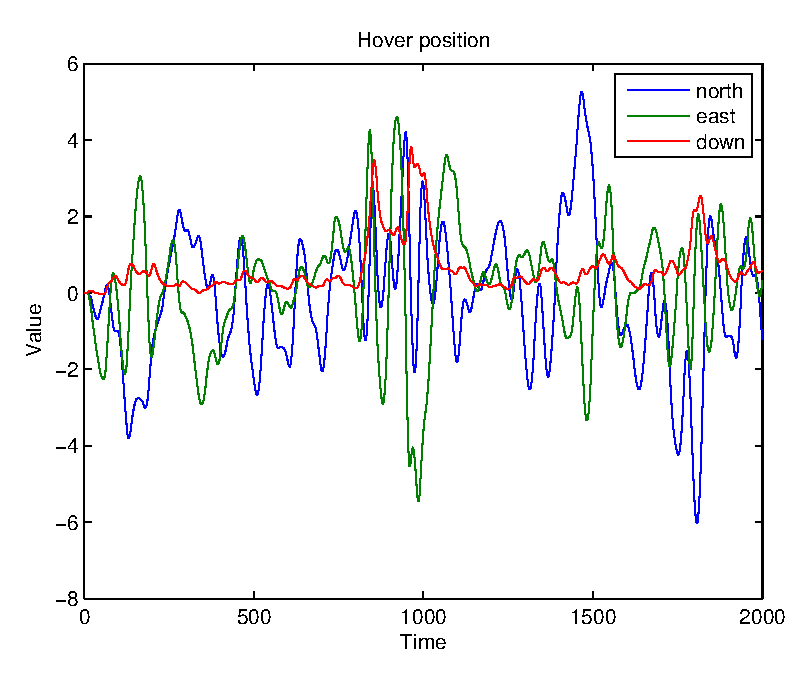
\includegraphics [width=4in]{Yujia_01.eps}



\end{document}
    
